\begin{figure*}

\begin{subfigure}{\textwidth}
\begin{minipage}[b]{0.7365\textwidth}
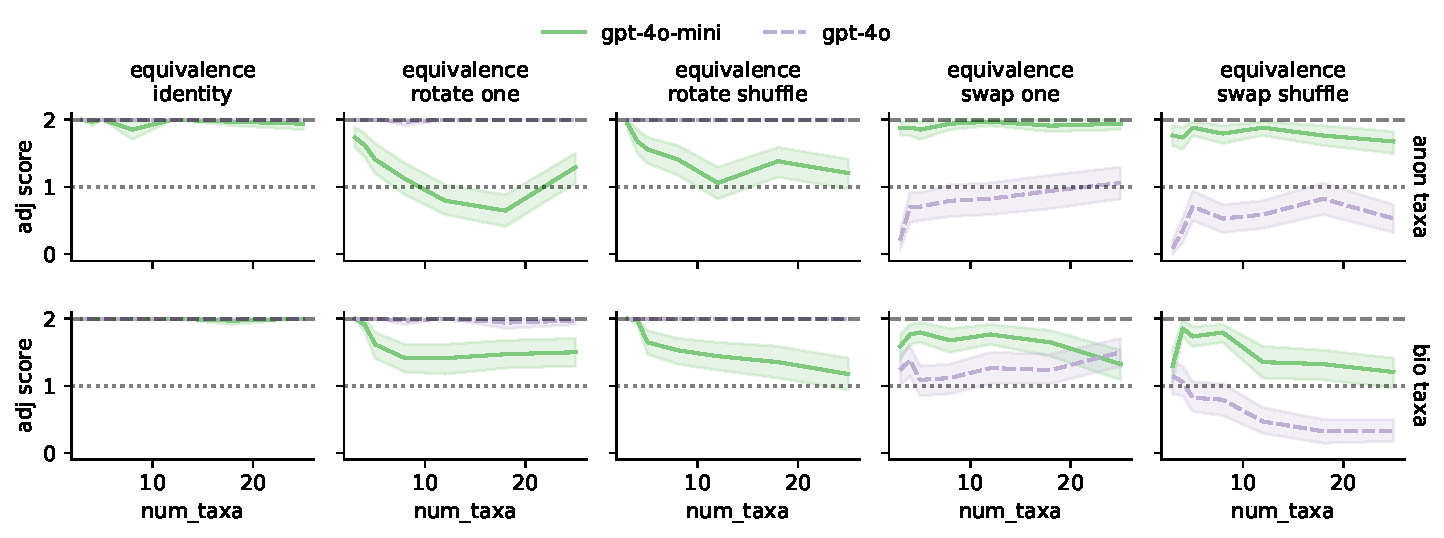
\includegraphics[width=\textwidth, trim={0cm 0cm 1cm 1cm}, clip]{binder/binder-2024-11-07-scientific.ipynb/binder/teeplots/2024-11-07-scientific/col=q+hue=model+is_equivalence=True+kind=line+palette=accent+repr_=json+row=tree-source+style=model+viz=relplot+x=num-taxa+y=adj-score+ext=.pdf}
\end{minipage}%
\begin{minipage}[b]{0.01\textwidth}
\end{minipage}
\begin{minipage}[b]{0.2535\textwidth}
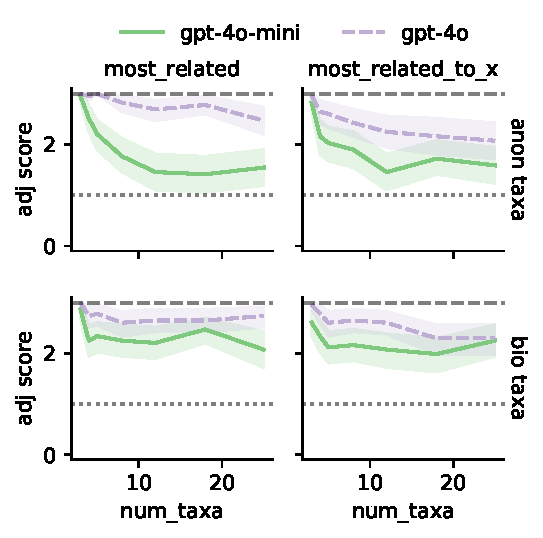
\includegraphics[width=\textwidth, trim={0.65cm 0cm 0cm 0cm}, clip]{binder/binder-2024-11-07-scientific.ipynb/binder/teeplots/2024-11-07-scientific/col=q+hue=model+is_equivalence=False+kind=line+palette=accent+repr_=json+row=tree-source+style=model+viz=relplot+x=num-taxa+y=adj-score+ext=.pdf}
\end{minipage}
\caption{\footnotesize JSON representation}
\label{fig:models:json}
\end{subfigure}

\begin{subfigure}{\textwidth}
\begin{minipage}[b]{0.7365\textwidth}
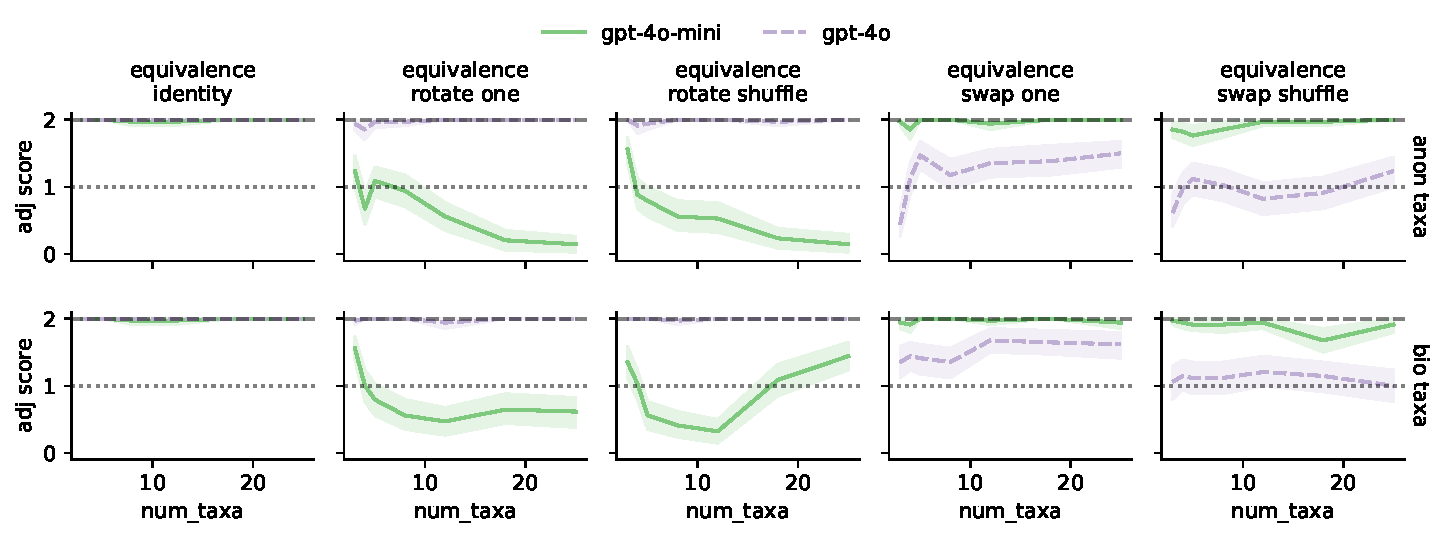
\includegraphics[width=\textwidth, trim={0cm 0cm 1cm 1cm}, clip]{binder/binder-2024-11-07-scientific.ipynb/binder/teeplots/2024-11-07-scientific/col=q+hue=model+is_equivalence=True+kind=line+palette=accent+repr_=newick+row=tree-source+style=model+viz=relplot+x=num-taxa+y=adj-score+ext=.pdf}
\end{minipage}%
\begin{minipage}[b]{0.01\textwidth}
\end{minipage}
\begin{minipage}[b]{0.2535\textwidth}
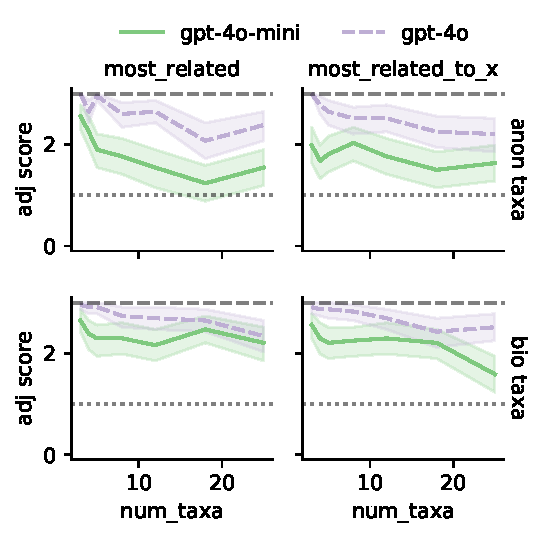
\includegraphics[width=\textwidth, trim={0.65cm 0cm 0cm 0cm}, clip]{binder/binder-2024-11-07-scientific.ipynb/binder/teeplots/2024-11-07-scientific/col=q+hue=model+is_equivalence=False+kind=line+palette=accent+repr_=newick+row=tree-source+style=model+viz=relplot+x=num-taxa+y=adj-score+ext=.pdf}
\end{minipage}
\caption{\footnotesize Newick representation}
\label{fig:models:newick}
\end{subfigure}

\begin{subfigure}{\textwidth}
\begin{minipage}[b]{0.7365\textwidth}
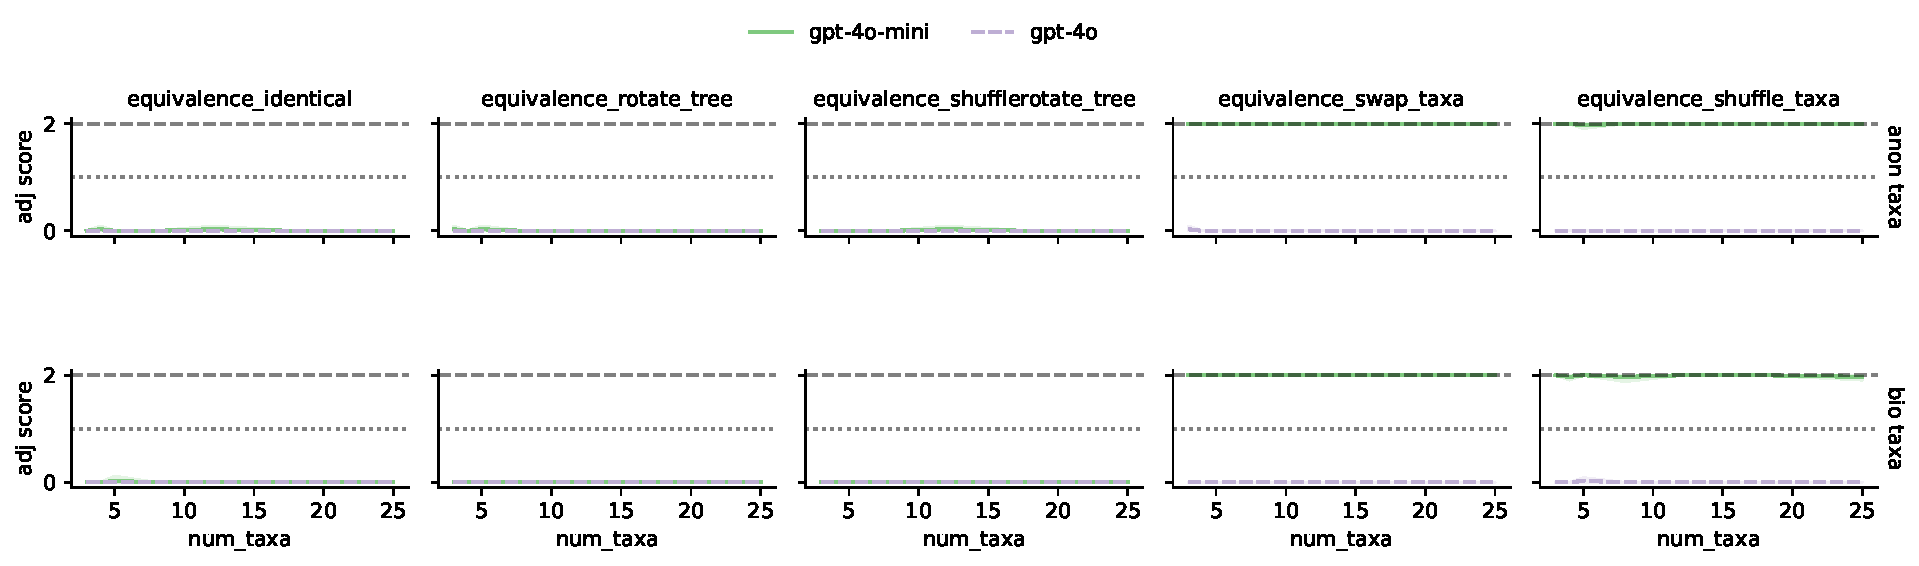
\includegraphics[width=\textwidth, trim={0cm 0cm 1cm 1cm}, clip]{binder/binder-2024-11-07-scientific.ipynb/binder/teeplots/2024-11-07-scientific/col=q+hue=model+is_equivalence=True+kind=line+palette=accent+repr_=none+row=tree-source+style=model+viz=relplot+x=num-taxa+y=adj-score+ext=.pdf}
\end{minipage}%
\begin{minipage}[b]{0.01\textwidth}
\end{minipage}
\begin{minipage}[b]{0.2535\textwidth}
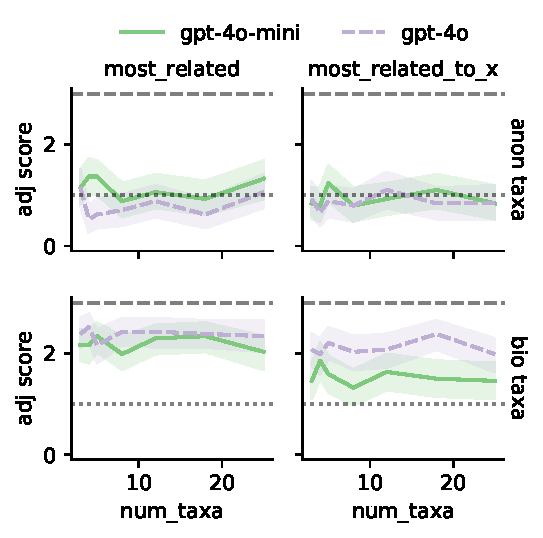
\includegraphics[width=\textwidth, trim={0.65cm 0cm 0cm 0cm}, clip]{binder/binder-2024-11-07-scientific.ipynb/binder/teeplots/2024-11-07-scientific/col=q+hue=model+is_equivalence=False+kind=line+palette=accent+repr_=none+row=tree-source+style=model+viz=relplot+x=num-taxa+y=adj-score+ext=.pdf}
\end{minipage}
\caption{\footnotesize Blank, no tree shown (control)}
\label{fig:models:blank}
\end{subfigure}

\caption{
\textbf{Tree thinking performance of surveyed large language models (LLMs).}
\footnotesize
Charts compare tree thinking test scores for OpenAI GPT-4o and OpenAI GPT-4o-mini.
Panels \cref{fig:models:blank,fig:models:newick,fig:models:json} compare prompts constructed using three tree rendeirng formats: Newick, JSON, or blank.
The third treatment is included as a control.
Adjusted score 1.0, indicated by dotted horizontal line, corresponds to expected correct responses under a random guessing strategy.
Dashed line at top of facets corresponds to best-possible performance, where all responses are correct.
Lattice rows differentiate prompts with ``anonymous'' trees, which were randomly generated with taxa identified as T0, T1, etc., and prompts with ``biological'' trees, which were subsampled from the Emoji tree of life \citep{mammola2023biodiversity} with taxa identified via binomial nomenclature (e.g., \textit{Panthera tigris}).
Note, in particular, that under the control ``blank'' tree treatment, biological taxa provide sufficient information to answer the ``most related'' and ``most related to $x$'' questions.
Shaded bands denote bootstrapped 95\% CI, $n=100$.
}
\label{fig:models}

\end{figure*}
